% Number 120
% BFPM Vectors Friction
% Force diagram MC on incline, bad lengths
% MIT Physics for Teachers LON-CAPA

% Watermark
\AddToShipoutPicture*{\BackgroundPic}

\addtocounter {ProbNum} {1}

\begin{floatingfigure}[r]{.3\textwidth}
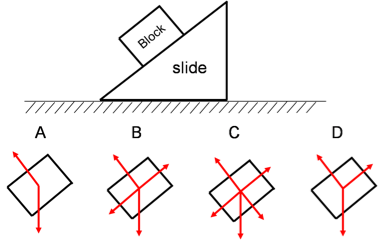
\includegraphics[scale=.4]{/Users/jgates/desktop/latex/pics/incline3.png}
\end{floatingfigure}
 
{\bf \Large{\arabic{ProbNum}}} A block sits at rest and stays at rest on a slide with frictional surfaces. Each red arrow represents a force. Observe their number and direction, but ignore their lengths.  

 \bigskip

\indent Which of the following sketches most closely resembles the correct free body diagram for all forces acting on the block? 

\vfill

\newpage
